\documentclass[a4paper,12pt, oneside]{article}

\usepackage[in]{fullpage}

\usepackage[utf8]{inputenc}
\usepackage[T1]{fontenc}
\usepackage[french]{babel}

\usepackage{amsmath}
\usepackage{amssymb}
\usepackage{mathtools}
\usepackage[inline]{enumitem}
\usepackage[squaren,Gray]{SIunits}
\usepackage{sistyle}
\usepackage[autolanguage]{numprint}
\usepackage{xfrac}
\usepackage{bm}
\usepackage{color}
\usepackage[version=3]{mhchem}
\usepackage{multirow}
\usepackage{tabulary}

\newcommand{\diff}[1]{\mathrm{d}#1}

\let\oldvec\vec
\renewcommand{\vec}[1]{\oldvec{\bm{#1}}}
\newcommand{\uvec}[1]{\hat{\bm{#1}}}

\newcommand{\TODO}[1]{\colorbox{red}{\textbf{\textsc{TODO: #1}}}}

\newcommand{\e}[1]{\ensuremath{\cdot 10^{#1}}}

\makeatletter
\newcommand\reaction@[1]{\begin{equation}\ce{#1}\end{equation}}
\newcommand\reaction@nonumber[1]%
{\begin{equation*}\ce{#1}\end{equation*}}
\newcommand\reaction{\@ifstar{\reaction@nonumber}{\reaction@}}
\makeatother

\title{Tâche 4 : Mini-Hazop}
\author{Groupe 1254}
\begin{document}
\maketitle
\section{Dangers des substances}
Premièrement, on retrouve dans la production d'ammoniac deux réactifs sous forme de gaz: l'azote, \ce{N2}, et l'hydrogène, \ce{H2}. Ces gaz ont la particularité d'être à la fois incolores et inodores. Le premier présente un danger de par le fait qu'il va "prendre la place" de l'oxygène présent dans l'air, provoquant ainsi un risque d'asphyxie (un taux d'oxygène inférieur à 19\% est létal). 
		
		L'hydrogène quant à lui est d'une part explosif (une fuite d'hydrogène augmentant donc grandement le risque d'incendies!) et d'autre part fortement corrosif envers les couches de fer composant les parois des réacteurs et reformeurs. Ainsi, ce composé crée des lèvres et des fissures dans lesdites parois, provoquant l'échappement des gaz présents dans le procédé chimique.
		
		En second lieu, l'ammoniac qui est lui aussi sous forme gazeuse, implique bien des risques. Bien qu'il soit facilement repérable grâce à son odeur particulière et prononcée (odeur repérable à partir de 5 ppm), il représente de gros risques pour la santé. En effet, une concentration d'\ce{NH3} comprise entre 400 et 700 ppm provoquera chez un inhalateur des irritations de la gorge variant en intensité tandis qu'une concentration de 10 000 ppm provoquera de graves conséquences médicales.

		Par ailleurs, l'ammoniac peut devenir explosif sous certaines conditions particulières de température et de pression. Il attaque également le zinc et le cuivre, nécessitant un équipement approprié lors de sa manipulation. Finalement, le \ce{NH3} présent sous l'état liquide s'évapore très rapidement lorsqu'il entre en contact avec de l'eau: il faudra donc pratiquer le spinning si nous sommes amenés à nettoyer une  flaque d'ammoniac.

\section{Circulation des flux de matière}  


Les flux et noeuds se trouvent aux figures~\ref{cir1},\ref{cir2},\ref{cir3}.
Le positionnement des noeuds se trouve à la figure~\ref{cir4}. Ces figures sont disponibles dans l'annexe \ref{Annexe Flux}

\section{Tableau de la mini-HAZOP}

(voir tableau excel)

\section{Soupape}
La réaction de production d'ammoniac du procédé que nous utilisons (\bsc{Haber} - \bsc{Bosch}) est la suivante:
$$\ce{N2 +3H2 <=> 2NH3}$$
Cette réaction est donc caractérisée par une diminution de moles de gaz. En nous rappelant la loi des gaz parfaits, on peut déduire que la réaction est aussi caractérisée par une diminution de pression. Il y a donc peu de risque d'une surpression dans le réacteur principal, rendant l'ajout d'une soupape et / ou d'un disque de rupture inutile.

\section{Disque de rupture}
L'eau chauffant, dans l'échangeur 124-MC, nous avons une augmentation de pression car $$pV=nRT$$ et que le nombre de mole reste constant. Cette pression augmentante entraîne alors un danger de suppression, un disque de rupture est alors nécessaire afin d'avoir une installation sécurisée.
L'eau chauffant nous avons une augmentation de pression car $$pV=nRT$$ et que le nombre de mole reste constant. Cette pression augmentante entraîne alors un danger de suppression, un disque de rupture est alors nécessaire afin d'avoir une installation sécurisée. 

\newpage
\appendix
\section{Circulation des flux de matière}

\label{Annexe Flux}

\begin{figure}[h]
	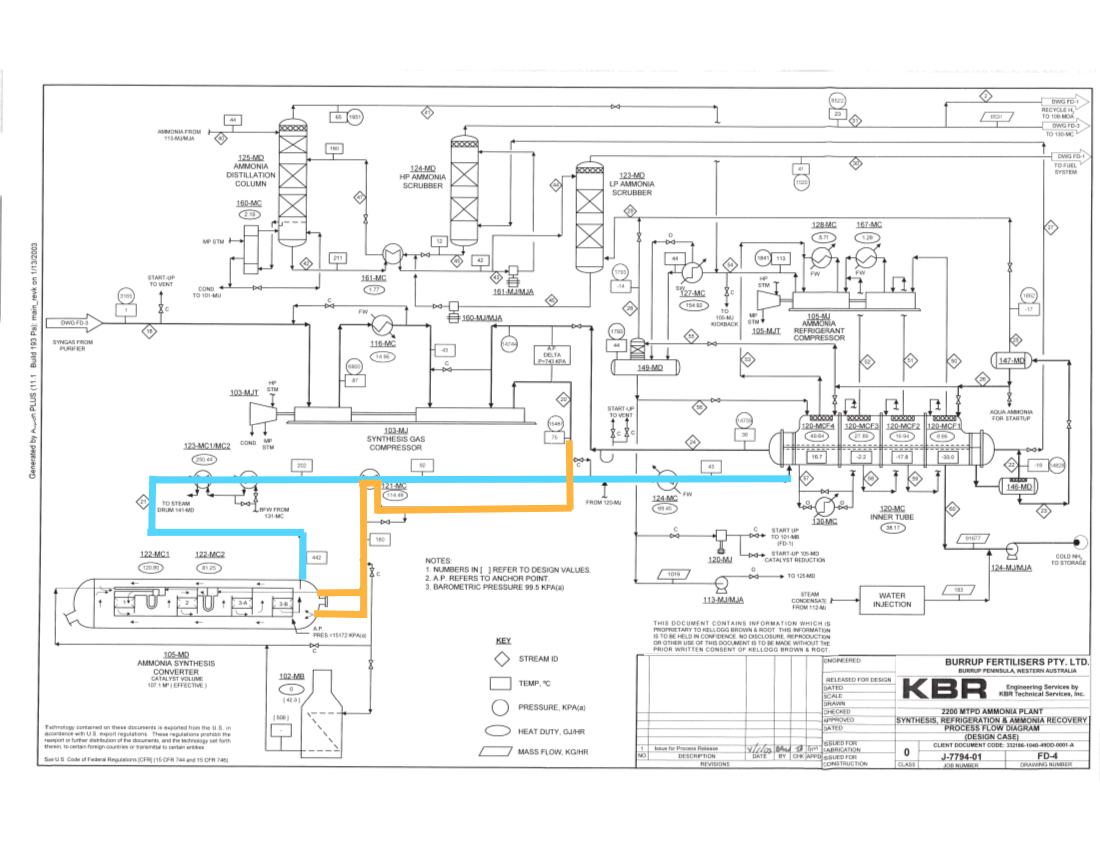
\includegraphics[scale=0.6]{Plan1.png}
	\caption{Circulation du flux}
	\label{cir1}
	\end{figure}
\begin{figure}[h]
	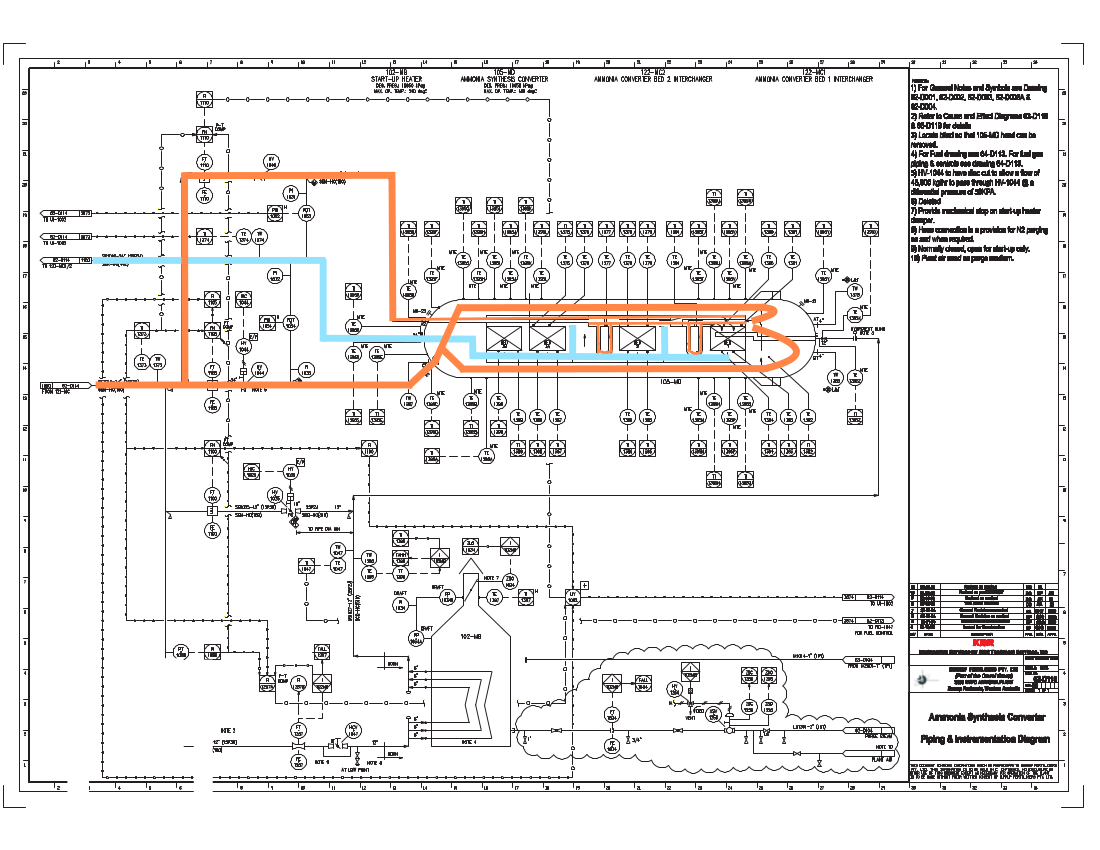
\includegraphics[scale=0.5]{Plan2.png}
	\caption{Circulation du flux}
	\label{cir2}
\end{figure}
\begin{figure}[h]
	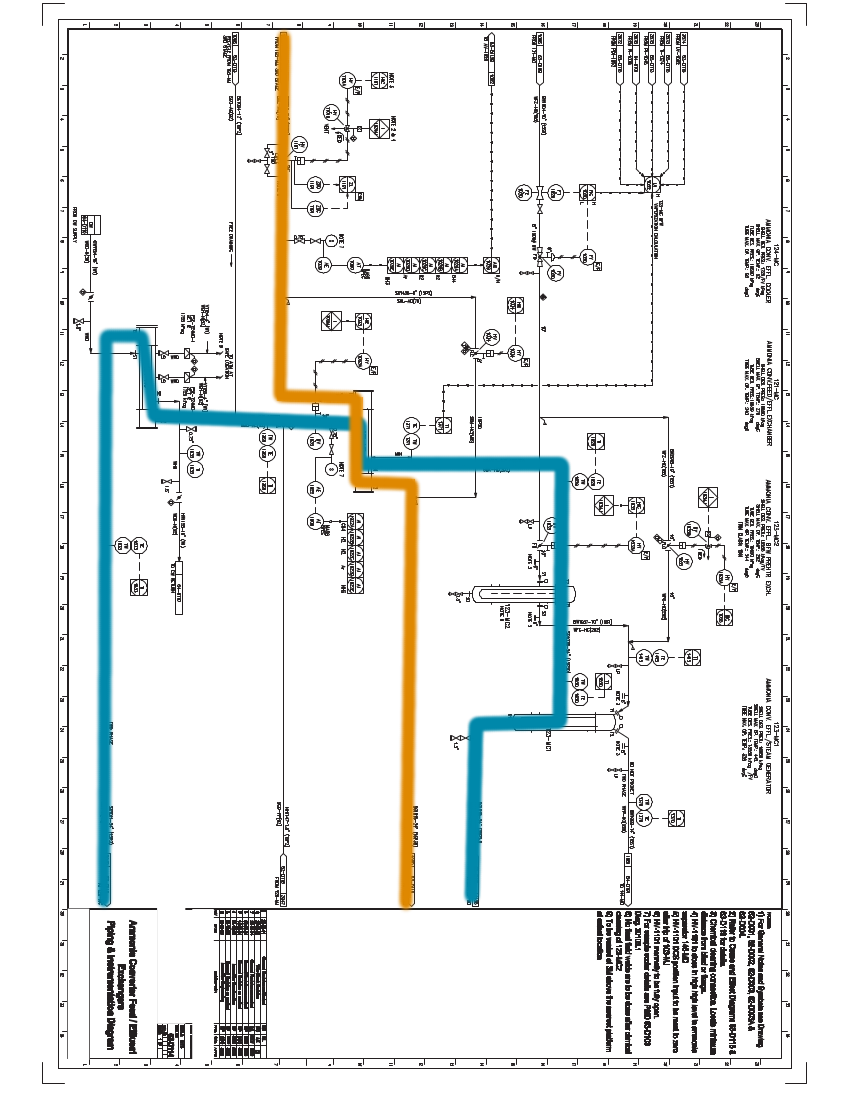
\includegraphics[scale=0.5]{Plan2-2.png}
	\caption{Circulation du flux}
	\label{cir3}
	\end{figure}
\begin{figure}[h]
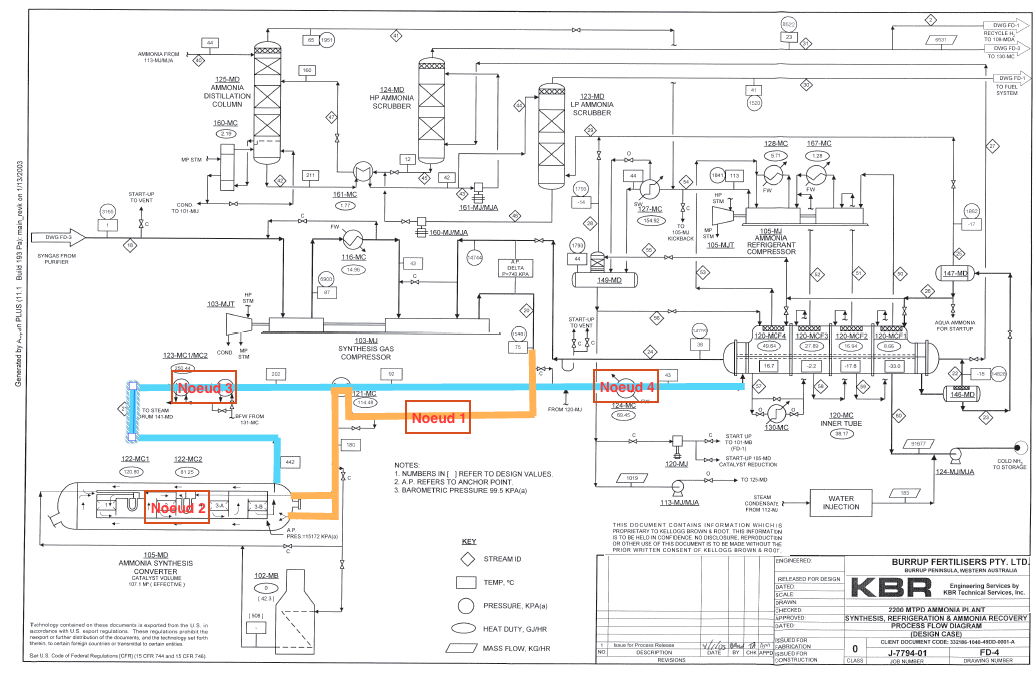
\includegraphics[scale=0.4]{Position_des_differents_noeuds.png} 
	\caption{Position des  Noeuds}
	\label{cir4}
\end{figure}

\end{document}